\section{Memory Map}
\label{sec:mem_map}

The memory map of the system, as seen by picoVersat programs, is given in
Table~\ref{tab:memmap}.

\begin{table}[!htbp]
  \centering
    \begin{tabular}{|p{3cm}|c|c|c|p{4cm}|}
    \hline 
    {\bf Mnemonic} & {\bf Address} & {\bf Read/Write} & {\bf Read Latency} & {\bf Description} \\
    \hline \hline 
     REGF\_BASE & 0x200 & Read+Write & 0 & Register file peripheral \\
    \hline
     CPRT\_BASE & 0x258 & Write only & NA & Debug printer periheral \\
    \hline
     LED\_BASE & 0x25A & Read+Write & 0 & Led peripheral \\
    \hline
     SWITCH\_BASE & 0x25C & Read only & 0 & Switch peripheral \\
    \hline
     BUTTON\_BASE & 0x25E & Read only & 0 & Button peripheral \\
    \hline
     DISPLAY\_BASE & 0x260 & Write only & 0 & Display peripheral \\
    \hline
     PS2\_BASE & 0x262 & Read only & 0 & PS2 peripheral \\
    \hline
     PROG\_BASE & 0x0 & Read+Write & 1 & User programs and data \\
    \hline
    \end{tabular}
  \caption{Memory map base addresses}
  \label{tab:memmap}
\end{table}

\clearpage
\section{Program Description}
\label{sec:pgrm}
The state diagram of the Fig.~\ref{fig:state}, it's the proposal system to implement, this diagram is intend to give an abstract description of the behavior of tthe system that will be running in the PicoVersat processor. This behavior is represented as a series of events that occur in the three states, and by this events the program will flow the schematic doing the value of the events.

\noindent
The idle state has the main objective of reset all the important variables of the system, after reseting the value of each led and the score of
the player, waits until the start button is pressed to initiate the game and call the state game.

\noindent
The game state is where the game occurs, this state has the main tasks such as sending the keystrokes to the verification state, if the verification flag is set to zero, the state will generate a new level and a new random sequence and the game will continue.

\noindent
The check state have the responsibility of checking each move and set the value of the check flag according to the value of received keys. Due the check flag the state will show the value of each level and score, if the flag last level is set to one the check state will return to the idle mode and send a message that the player have won the game.

\begin{figure}[!htbp]
    \centerline{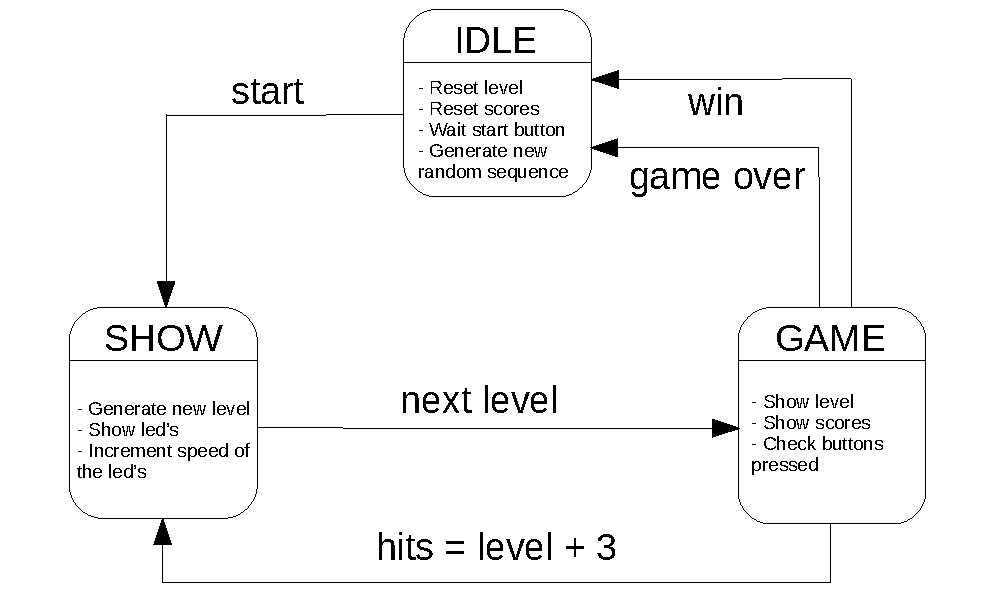
\includegraphics[width=\textwidth]{state}}
    \vspace{0cm}\caption{State diagram}
    \label{fig:state}
\end{figure}
